\showtocfalse

\begin{document}

%----------------------------------------------------------------------------------------
%	TITLE PAGE
%----------------------------------------------------------------------------------------

\title[3 Types of FL]{Three Types of Federated Learning}
\date{}

% \institute[北京航空航天大学] % Your institution as it will appear on the bottom of every slide, maybe shorthand to save space
% {
% 数学科学学院 \\ % Your institution for the title page
% \medskip
% \textit{wenh06@gmail.com} % Your email address
% 北京航空航天大学 \\
% 数学科学学院 \qquad 北京航空航天大学
% }

% \date{\footnotesize 2023年1月10日} % Date, can be changed to a custom date

\setlength{\belowdisplayskip}{5pt} \setlength{\belowdisplayshortskip}{5pt}
\setlength{\abovedisplayskip}{5pt} \setlength{\abovedisplayshortskip}{5pt}

%------------------------------------------------

\begin{frame}
\titlepage % Print the title page as the first slide
\end{frame}

%------------------------------------------------
% Page 1

\begin{frame}
\frametitle{Horizontal Federated Learning}

\begin{align*}
    & \text{minimize} \quad f(\theta) = \expectation\limits_{k \sim {\mathcal{P}}} [f_k(\theta)] = \sum_{k=1}^K w_k f_k(\theta) \\
    & \text{where} \quad f_k(\theta) = \expectation\limits_{(x, y) \sim \mathcal{D}_k} [\ell_k(\theta; x, y)]
\end{align*}

\begin{itemize}
\item $\theta:$ learning objective (model parameters),
\item $\mathcal{P}:$ distribution of clients,
\item $w_k:$ weight of client $k$,
\item $\mathcal{D}_k \subseteq \mathcal{X}_k \times \mathcal{Y}_k:$ distribution of data on client $k$,
\begin{itemize}
    \item $\mathcal{X}_k:$ feature distribution,
    \item $\mathcal{Y}_k:$ label distribution,
\end{itemize}
\textbf{underlying feature spaces and label spaces are the same across clients.}
\item $\ell_k:$ loss function.
\end{itemize}

\end{frame}

%------------------------------------------------
% Page 2

\begin{frame}
\frametitle{Vertical Federated Learning}

{\smaller
\begin{align*}
    & \text{minimize} \quad f(\theta) = {\color{cyan} \sum_{i=1}^N} \mathcal{L} \left( {\color{red} \mathcal{F}_K}\left( {\color{red} \varphi_K}; f_{\color{purple} 1}(\theta_{\color{purple} 1}; x_{\color{cyan} i}^{\color{purple} (1)}), \ldots, f_{\color{purple} K}(\theta_{\color{purple} K}; x_{\color{cyan} i}^{\color{purple} (K)}), y_{\color{cyan} i} \right) \right) \\
    & \text{where} \quad \theta = (\theta_{\color{purple} 1}, \ldots, \theta_{\color{purple} K}), ~ x_{\color{cyan} i} = (x_{\color{cyan} i}^{\color{purple} (1)}, \ldots, x_{\color{cyan} i}^{\color{purple}(K)})
\end{align*}
}

\begin{block}{A Simple Example: Group Lasso}
\begin{align*}
\beta^{\ast} & = \operatorname*{argmin}_{{\color{purple} \beta}} \left\{ \left\lVert {\color{cyan} y} - \sum_{k=1}^{K} {\color{cyan} X^{(k)}} {\color{purple} \beta^{(k)}} \right\rVert_2^{2} + \lambda \sum_{k=1}^{K} \left\lVert {\color{purple} \beta^{(k)}} \right\rVert_2 \right\}
\end{align*}
\end{block}

\blfootnote{\tiny \cite{Liu_2022_FedBCD}\bibentry{Liu_2022_FedBCD}}

\end{frame}

%------------------------------------------------
% Page 2

\begin{frame}
\frametitle{Vertical Federated Learning}

\begin{figure}
\centering
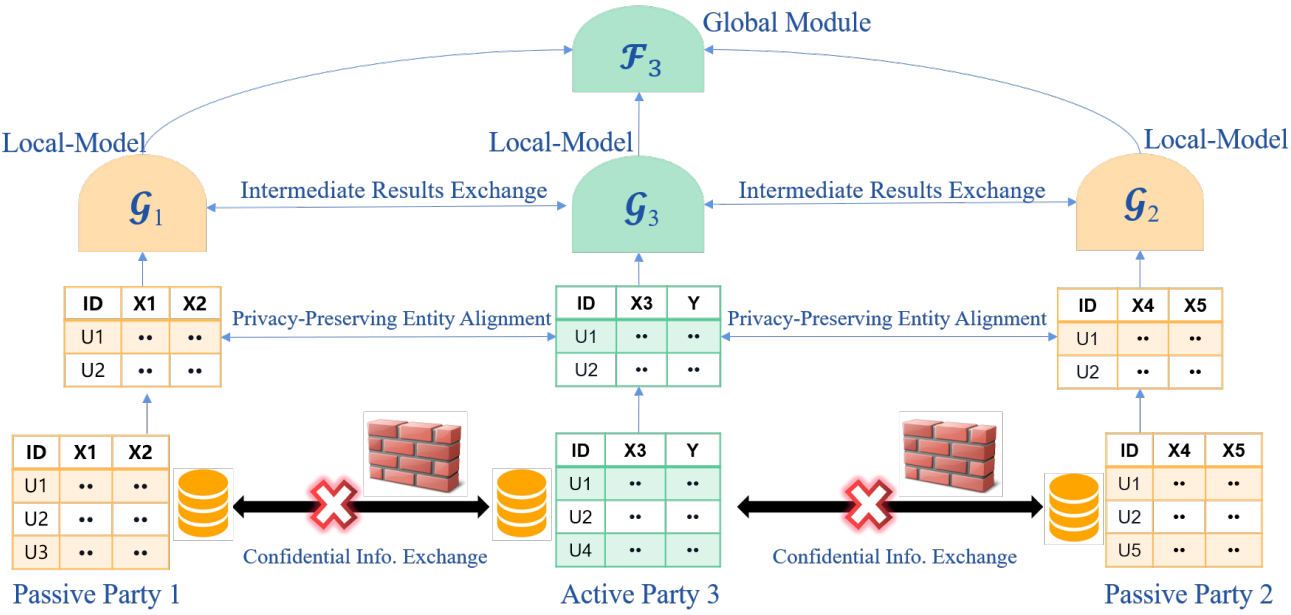
\includegraphics[width=\textwidth,keepaspectratio]{images/vfl.png}
\end{figure}

\blfootnote{\tiny 图片来源:\cite{vfl}\bibentry{vfl}}

\end{frame}

%------------------------------------------------
% Page 4

\begin{frame}
\frametitle{Federated Transfer Learning}

\begin{figure}
\centering
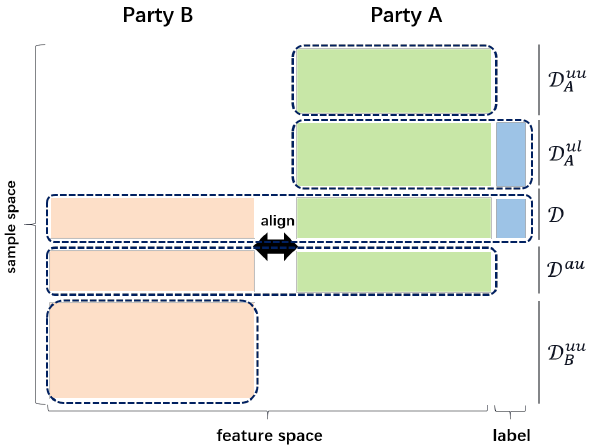
\includegraphics[width=0.45\textwidth,keepaspectratio]{images/transfer-fl.png}
\end{figure}

One choice \cite{liu_2020_transfer_fl} is to map feature space A and B to some common feature space $U$, and solve
$$
\text{minimize} \quad \sum_{k=1}^{K_{AB}} \left( \ell_1(y_k^A, {\color{red} \varphi}(u_k^B)) + \lambda {\color{red} \ell_2}(u_k^A, u_k^B)  \right)
$$

\blfootnote{\tiny \cite{liu_2020_transfer_fl}\bibentry{liu_2020_transfer_fl}}

\end{frame}

%------------------------------------------------
% Page 5

\begin{frame}
\frametitle{Visualization}

% 从左到右依次是横向联邦学习,纵向联邦学习,迁移联邦学习
\begin{columns}

\begin{column}{0.26\textwidth}
\begin{figure}
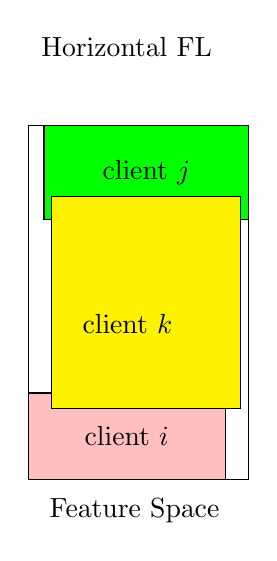
\begin{tikzpicture}
\draw (0,0) rectangle (2.8,4.5);
\node at (1.25,5.5) {Horizontal FL};
\draw[fill=pink] (0,0) rectangle (2.5,1.1) node[pos=.5] {client $i$};
\draw[fill=green] (0.2,3.3) rectangle (2.8,4.5) node[pos=.5] {client $j$};
\draw[fill=yellow] (0.3,0.9) rectangle (2.7,3.6) node[pos=.4] {client $k$};
\node at (1.35,-0.4) {Feature Space};
\end{tikzpicture}
\end{figure}
\end{column}

\begin{column}{0.26\textwidth}
\begin{figure}
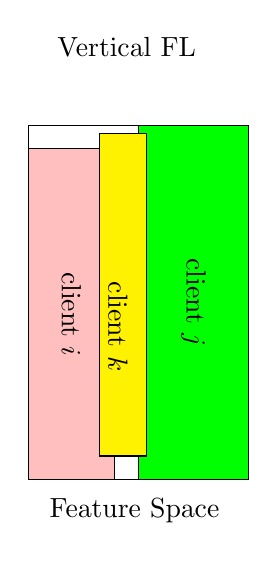
\begin{tikzpicture}
\draw (0,0) rectangle (2.8,4.5);
\node at (1.25,5.5) {Vertical FL};
\draw[fill=pink] (0,0) rectangle (1.1,4.2) node[pos=.5,rotate=-90] {client $i$};
\draw[fill=green] (1.4,0) rectangle (2.8,4.5) node[pos=.5,rotate=-90] {client $j$};
\draw[fill=yellow] (0.9,0.3) rectangle (1.5,4.4) node[pos=.4,rotate=-90] {client $k$};
\node at (1.35,-0.4) {Feature Space};
\end{tikzpicture}
\end{figure}
\end{column}

\begin{column}{0.26\textwidth}
\begin{figure}
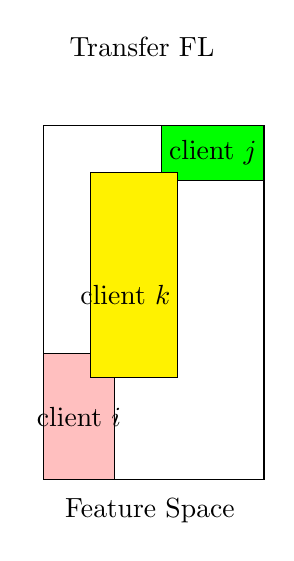
\begin{tikzpicture}
\draw (0,0) rectangle (2.8,4.5);
\node at (1.25,5.5) {Transfer FL};
\draw[fill=pink] (0,0) rectangle (0.9,1.6) node[pos=.5] {client $i$};
\draw[fill=green] (1.5,3.8) rectangle (2.8,4.5) node[pos=.5] {client $j$};
\draw[fill=yellow] (0.6,1.3) rectangle (1.7,3.9) node[pos=.4] {client $k$};
\node at (1.35,-0.4) {Feature Space};
\end{tikzpicture}
\end{figure}
\end{column}

\begin{column}{0.13\textwidth}
\begin{figure}

\begin{tikzpicture}
% \coordinate (sample_node) at (0,0);
% \node[text width=1, left=0.5cm of sample_node.west] at () {样本维度};
\node[rotate=-90] () {Sample ID Space};
\end{tikzpicture}
\end{figure}
\end{column}

\end{columns}

\end{frame}

%------------------------------------------------
% Page 5

\begin{frame}[allowframebreaks]
\frametitle{References}

{\footnotesize
\bibliographystyle{ieeetr}
\bibliography{references}
}

\end{frame}

\end{document}
